%\documentclass{article} %[twocolumn] 
%\documentclass[Crown, times, sagev]{sagej}
\documentclass[sagev, Crown]{sagej} %

%\usepackage{algorithmic}
\usepackage{algorithm}
\usepackage{algorithmicx}
\usepackage{algpseudocode}
\usepackage{booktabs}
\usepackage{array}
\usepackage{graphicx}
\usepackage{amsmath}
\usepackage{amsfonts}
\usepackage{amssymb}
\usepackage{amsthm}
\usepackage{multirow}
\usepackage{url}

\setcounter{secnumdepth}{3} %Gives section numbers for cross referencing

\newtheorem*{mydef}{Definition}

\begin{document}

\runninghead{Wilson et al.}

\title{Optimising error rates in programmes of pilot and definitive trials using Bayesian statistical decision theory}

\author{Duncan T. Wilson\affilnum{1}}%,
%Rebecca E. A. Walwyn\affilnum{1}, 
%Julia Brown\affilnum{1} and 
%Amanda J. Farrin\affilnum{1}}

\affiliation{\affilnum{1}Leeds Institute of Clinical Trials Research, University of Leeds, Leeds, UK} %\\
%\affilnum{2}Centre for Primary Care \& Public Health, Queen Mary University of London, London, UK}

\corrauth{Duncan T. Wilson, Clinical Trials Research Unit, Leeds Institute of Clinical Trials Research, University of Leeds, Leeds, LS2 9JT, UK}
\email{d.t.wilson@leeds.ac.uk}

\begin{abstract}
% (300 word limit for ICTMC) (250 limit for SiM)
Pilot trials of complex interventions are often conducted in advance of definitive trials to assess feasibility and to inform their design. Although pilot trials typically collect primary endpoint data, preliminary tests of effectiveness have been discouraged given their low power resulting from the small pilot sample size and assuming a conventional type I error rate. Power could be increased at the cost of a higher type I error rate, but there is little methodological guidance on how to determine the optimal balance between these factors. We consider a Bayesian decision-theoretic approach to this problem, introducing a utility function and defining an optimal pilot and definitive trial programme as that which maximises expected utility. We base utility on changes in average primary outcome, the cost of sampling, treatment costs, and the decision-maker's attitude to risk. We apply this approach to re-design OK-Diabetes, a pilot trial of a complex interventions with a continuous primary outcome with known standard deviation. We then examine how optimal programme characteristics vary with the parameters of the utility function. We find that the conventional approach of not testing for effectiveness in a pilot trial can be considerably sub-optimal.
\end{abstract}

\keywords{Clinical trial, pilot trial, external pilot, statistical decision theory, optimal design, expected utility}

\maketitle

% approx 6163 words, 2 tables and 5 figures (6163 + 7*200 = 7563, SMMR asks for around 8k)

\section{Introduction}

Pilot trials are a type of feasibility study which take the same form as a planned definitive trial of a complex intervention, but on a smaller scale \cite{Eldridge2016}. Internal pilots constitute the initial phase of the definitive trial,  with the pilot data being used in the final analysis. In contrast, external pilots are conducted separately to the definitive trial, with a clear gap between the two stages. A key goal of any pilot trial is to guide the decision of whether or not the definitive trial should go ahead, typically with a focus on feasibility issues such as recruitment rates and levels of missing data \cite{Craig2008, Thabane2010, Eldridge2016a}.

Although pilot trials will generally collect data measuring the effectiveness of the intervention, assessing effectiveness at the pilot stage has been discouraged due to concerns that the small pilot sample size will provide low power and lead to effective interventions being incorrectly discarded \cite{Lancaster2004, Arain2010, Westlund2016, Sim2019}. This criticism rests on two assumptions. Firstly, it assumes that the pilot and definitive trials will share a primary endpoint, with the same minimal clinically important difference (MCID). Secondly, it assumes that any pilot trial hypothesis test will be conducted with a significance level in the conventional range of 0.01 - 0.1. For example, an two-arm parallel group external pilot trial with a normally distributed primary endpoint designed using the rule-of-thumb of 35 participants per arm \cite{Teare2014} would have a power of 23\% (or equivalently, a type II error of $\beta = 0.77$) to detect a standardised effect size of 0.3 when using a one-sided type I error rate of $\alpha = 0.025$.

While the assumption of a constant MCID will often hold, there is no obvious reason for type I error rates in pilots to be constrained at conventionally low levels. Indeed,
by not testing at all we effectively obtain a procedure with error rates $\alpha = 1, \beta = 0$. This testing strategy is only optimal if we have an absolute preference for minimising type II errors over type I errors in the pilot, a preference too extreme to be expected in practice. As illustrated in Figure \ref{fig:ocs}, it will often be possible to reduce $\alpha$ considerably (in this case, from 1 to 0.75) at the cost of only a small increase in $\beta$ (from 0 to 0.027). Although relaxing the type I error rate in a pilot has been suggested before \cite{Cocks2013, Lee2014}, there is a lack of methodological guidance for determining exactly how much it should be relaxed by, or for choosing an appropriate pilot sample size. 

\begin{figure}
\centering
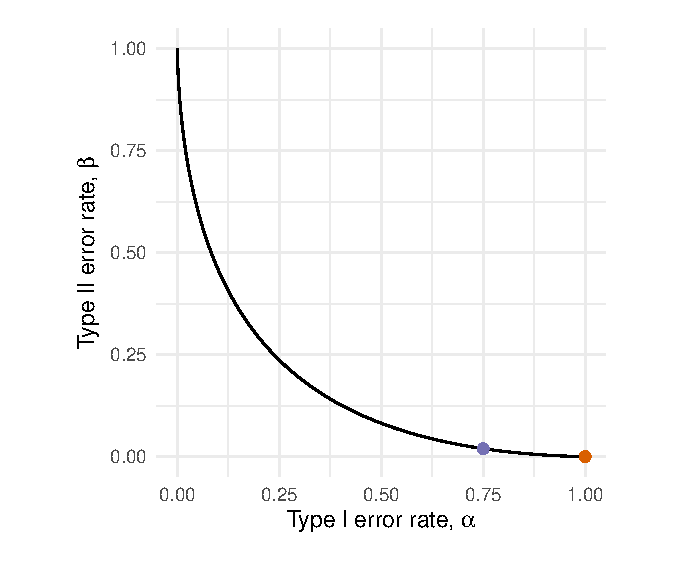
\includegraphics[scale=0.8]{./figures/ocs.eps}
\caption{Operating characteristic curves for an external pilot trial testing efficacy.}
\label{fig:ocs}
\end{figure} 

One possible approach to defining optimal error rates is through Bayesian statistical decision theory. Under this framework we define a suitable utility function which encodes our preferences, and make decisions based on the expected value of this utility with respect to a prior distribution which expresses our uncertainty on the unknown parameters. Although the theory is well established \cite{Raiffa1961, Keeney1976, Lindley1997} and has been proposed in much methodological work around optimal trial design \cite{Hee2016}, it has been argued that the requirement of specifying a utility function has led to low uptake in practice \cite{Joseph1997a}. 

In this paper we aim to propose a simple and general form for a utility function in clinical trials, making clear the assumptions which are encoded in it and thus allowing its applicability or otherwise to the problem at hand to be judged. The utility we propose is closely related to several existing proposals in the literature \cite{Pearce2018}, but with some key differences. One particular aspect we have considered is the decision-maker's attitude to risk, an issue sidestepped by many exiting proposals which assume, explicitly or implicitly, that the decision-maker is risk-neutral. We will show that the attitude to risk can have a considerable effect on decision making, and is key to answering one of the motivating questions of this paper: in what situations, if any, is it optimal to \emph{not} test effectiveness in a pilot trial?

The remainder of this paper is structured as follows. We define the specific problem under consideration in Section \ref{sec:problem}, and describe the proposed method in Section \ref{sec:methods}. In Section \ref{sec:illustration} we illustrate the application of the method to design an external pilot of a complex intervention. We evaluate the properties of the method over a range of possible scenarios in Section \ref{sec:evaluation}, and then outline some extensions in Section \ref{sec:extensions}. Finally, we conclude with a discussion of the strengths and limitations of the proposed approach in Section \ref{sec:discussion}.

% Ref to VoI lit

\section{Problem}\label{sec:problem}

Consider the problem of jointly designing an external pilot trial and subsequent definitive trial. We will denote these, respectively, as stages $i=1$ and $i=2$ of the overall programme. We consider the case where both trials are parallel group studies comparing an intervention to control. We assume that the comparison focusses on superiority in terms of the mean difference of a normally distributed primary endpoint with known standard deviation common to each arm, where the same endpoint is used in both the pilot and definitive trials (although see Section \ref{sec:extensions} for relaxations of some of these assumptions). 

We denote the true mean difference by $\mu$, and consider the case where the the primary analysis at each stage will be a test of the null hypothesis $H_0: \mu = 0$. The test at stage $i$ will compare the sample mean difference between groups, denoted  $x_i$, to a pre-specified critical value, denoted $d_i$. At the pilot stage, a positive result (i.e. $x_1 > d_1$) will indicate that we should proceed to the definitive trial. At the definitive stage, a positive result (i.e. $x_2 > d_2$) will indicate that the intervention should be recommended for use over the control treatment. The thresholds $d_1, d_2$, along with the per-arm sample sizes at each stage $n_1, n_2$, collectively define the design of the overall programme. The design problem we consider in this paper is to optimise $n_i, d_i, i = 1,2$.

Given some alternative hypothesis $H_1: \mu =\mu^*$, we define the type I and II error rates for stage $i$ in the usual way, i.e. $\alpha_i = Pr[x_i > d_i \mid \mu = 0]$ and $\beta_i = Pr[x_i \leq d_i \mid \mu = \mu^*]$. An alternative summary of the pilot and definitive trial programme is then  $\alpha_i, \beta_i, i=1,2$.

% to add - full, explicit likelhood model

\section{Maximising expected utility in trial programmes}\label{sec:methods}

We consider a Bayesian view of the frequentist design problem, and therefore require a prior distribution for the unknown true mean difference $\mu$. This prior information will be used only to guide the choice of the frequentist design and analysis parameters, and not in any analysis of the trial data itself. As such, a non- or weakly-informative prior is not appropriate; rather, the prior should be a subjective summary of the decision-maker's knowledge and uncertainty about $\mu$. For computational tractability we will assume a conjugate normal prior $p(\mu)$ with mean $m_0$ and variance $s^2$.

We define optimal design variables as those which maximise the expectation, with respect to the prior $p(\mu)$, of a utility function. We construct the utility function in three steps, following the procedures described by Keeney and Raiffa \cite{Keeney1976}. First, we identify the \emph{attributes} which we consider will be of interest to the decision maker. We then define a \emph{value function} over the space of these attributes, which encodes the decision-maker's preferences under conditions of certainty. We then transform this value function into a \emph{utility function} by incorporating the decision-maker's attitude to risk. Throughout, we will make explicit the assumptions which are implied by the parametric forms of the value and utility functions, returning to discuss their implications in Section \ref{sec:discussion}.

\subsection{Attributes}

The first attribute of interest is the change in average outcome for the patient population, in terms of the primary endpoint, after the trial programme has been conducted. We denote this change by $d$. It will be determined by three factors: the trial outcomes (in terms of the binary hypotheses test results); the true treatment difference $\mu$; and the manner in which patients adopt the new treatment if the definitive trial concludes it is effective. Considering the latter requires a model predicting how patients will choose treatments. For simplicity, we will use a simple model assuming that the whole population will adopt the new treatment if the result of the definitive trial is positive, leading to a change in outcome of $d = \mu$. Otherwise, the population will retain the control treatment and the change in outcome will be $d=0$.

The sample size at both stages of the programme is of interest, being associated with both monetary costs and the exposure of patients to research. The total sample size will vary from programme to programme, both by design and through the uncertain outcome of the pilot trial. Assuming that sampling at each stage is equivalent in terms of the costs involved, we can then identify the total sample size $n = n_1 + n_2$ as our second attribute. 

While the focus of comparison between the intervention and control is in terms of the primary outcome, the treatments will in general differ in other aspects. We limit ourselves to the case where these differences are deterministic and known, and will refer to them as the treatment costs associated with the intervention. In this case, we can encapsulate these differences in a single indicator variable, and our third attribute,  $C \in \{0, 1\}$ where $C = 0$ if and only if a positive result is obtained in the definitive trial. 

\subsection{Value}

Considering preferences under conditions of certainty, we use the notation $y \prec y'$ to mean $y$ is preferred to $y'$, and $y \sim y'$ to mean indifference between $y$ and $y'$. We assume that $\prec$ is a weak ordering (i.e. complete and transitive) of all possible values $y$. We aim to specify a value function $v(n, C, d)$ which will assign to each possible set of attribute values a real number (its \emph{value}) which corresponds with the qualitative preferences of the decision maker. That is, we require $v(n, C, d)$ such that
$$
(d, n, C) \prec (d', n', C') \Leftrightarrow v(d, n, C) < v(d', n', C')
$$
for all $(d, n, C), (d', n', C')$. We will use a value function with the following additive form:
$$ 
v(d, n, C) =  v_d(d) + v_n(n) + v_c(C),
$$
where $v_d, v_n$ and $v_c$ are value functions representing preferences over each of the attributes when considered in isolation. It has been shown that such an additive value function exists if and only if each pair of attributes is \emph{preferentially independent} of the remaining attribute.

\begin{mydef}[Preferential independence  \cite{Keeney1976} (page 101)] %\cite[p.~101]{Keeney1976}]
 The pair of attributes $X$ and $Y$ is preferentially independent of attribute $Z$ if $(x', y', z) \prec (x'', y'', z) \Longleftrightarrow  (x', y', z') \prec (x'', y'', z')$ for any $z, z'$.
\end{mydef}

This condition requires, for example, that attributes $n$ and $C$ are preferentially independent of attribute $d$ in the sense that preferences on the $(n, C)$ space for a fixed $d'$ do not depend on the specific value of $d'$.

We impose further structure on the value function by assuming the single-attribute functions $ v_d(d)$ and  $v_n(n)$ are linear in their arguments. This implies a very specific preference structure, where the value of a change in attribute level from $d'$ to $d' + \Delta$ is independent of the starting level $d'$; and likewise for attribute $n$. Attribute $C$ only has two levels and therefore $v_c$ does not require any further specification. For ease of notation we will use the following single-attribute value functions:
$$ 
v_d(d) = k_d d, ~ v_n(n) = k_n n, ~ v_C(C) = k_c C.
$$
We elicit the scaling parameters $k_d, k_n$ and $k_c$ as follows. First, we ask the decision-maker to specify a change in outcome $\bar{d}$ that would justify increasing the total sample size from 0 to some value $n^*$. That is, we require $\bar{d}$ such that
$$
(d = 0, n = 0, C = 1) \sim (d = \bar{d}, n = n_*, C = 1).
$$
Note that the linear nature of $v_n$ and $v_d$ mean the specific choice of $n_*$ is arbitrary. Secondly, we ask for the change in outcome $\hat{d}$ that would justify switching from the current standard treatment to the intervention under study. That is, we require $\hat{d}$ such that
$$
(d = 0, n, C = 1) \sim (d = \hat{d}, n, C = 0).
$$
Finally, since value functions are invariant under linear transformations, we can set $k_n + k_c + k_d = 1$ and are left with the following system of equations:
\begin{align*}
k_d \bar{d} + k_n n_* &= 0 \\
k_d \hat{d} - k_c &= 0 \\
k_d + k_n + k_c &= 1
\end{align*}
This gives the following scaling parameters:
\begin{equation}\label{eqn:ks}
k_d = 1/(1 + \hat{d} - \bar{d}/n_*), ~ k_n = -k_d \bar{d}/n_* , ~ k_c = k_d \hat{d}. 
\end{equation}

\subsection{Utility}

The value function represents preferences under conditions of certainty, but in reality we are uncertain about the true values of all three attributes. To accommodate this uncertainty, we move from a value function to a utility function. This allows us to compare probability distributions over the attribute space, as opposed to only fixed points, and make decisions by choosing the distribution which has the largest expected utility.

To define the form of our utility function, we first argue that the change in outcome $d$ is \emph{utility independent} of the other two attributes, $n$ and $C$. 

\begin{mydef}[Utility independence  \cite{Keeney1976} (page 226)] %\cite[p.~226]{Keeney1976}]
Attributes $Y$ is utility independent of attribute $Z$ when conditional preferences for lotteries on $Y$ give $z'$ do not depend on the particular level of $z'$.
\end{mydef}

This means that regardless of how much we have sampled, or whether or not we have incurred the treatment costs associated with the intervention, our preferences for gambles on the change in outcome will be the same. Given this assumption together with the additive form of the value function, the utility function must have one of the following forms \cite{Keeney1976} (page 330):
\begin{equation}\label{eqn:expo_util}
u(n, C, d) =
\begin{cases}
1 - e^{-\rho v(n, C, d)}, &\rho > 0 \\
v(n, C, d), &\rho = 0 \\
-1 + e^{-\rho v(n, C, d)}, &\rho < 0 
\end{cases}
\end{equation}
A value of $\rho = 0$ implies a risk-neutral attitude, whereas $\rho$ greater than (less than) 0 implies a risk-averse (risk-seeking) attitude. To elicit $\rho$ we first note that we can think about gambles on $d$ whilst ignoring the value of the other attributes, since $d$ is utility independent of $n$ and $C$. We then elicit the value $d^*$ such that we would be indifferent between the following:
\begin{enumerate}
\item Obtaining $d^*$ with certainty;
\item A gamble which will result in $d_{min}$ with probability 0.5 and $d_{max}$ with probability 0.5.
\end{enumerate}
That is, we find $d^*$ such that
$$
u(n, C, d^*) = 0.5u(n, C, d_{min}) + 0.5u(n, C, d_{max}).
$$
In the special case of risk-neutrality, $\rho = 0 \Leftrightarrow d^* = 0.5d_{min} + 0.5d_{max}$. For $\rho \neq 0$ we have
$$
d^* = - \frac{1}{\rho} \ln\left( 0.5e^{-\rho d_{min}} + 0.5e^{-\rho d_{max}} \right),
$$
and so we can determine $\rho$ given $d^*$. For example, setting (arbitrarily) $d_{min} = 0, d_{max} = 1$, a value of $\rho = 2$ corresponds with $d^* =  0.283$. That is, $\rho = 2$ implies an indifference between obtaining a guaranteed change in outcome of 0.283, and a simple 50/50 gamble between no change at all and a change of 1. 

\subsection{Expected utility}

Denote by $G_i \in \{0, 1\}$ an indicator variable where $G_i = 1$ if there is a positive test result at stage $i$, and $G_i = 0$ otherwise. For the problem considered here, $G_i = 1 \Leftrightarrow x_i > d_i$. Noting that the attributes $d$, $n$ and $C$ are completely determined by the fixed programme design $z$, the realisations of $G_1$ and $G_2$, and the true treatment effect $\mu$, we re-write utility as $u(\mu, G_1, G_2 ~|~ z)$. Focussing on the case where $\rho > 0$ (the other cases will follow), we have
\begin{equation}
\begin{split}
u(\mu, G_1, G_2 ~|~ z) = 1 - \exp(&-\rho[k_d\mu + k_n (n_1+n_2)] G_1 G_2 \\ 
  &- \rho[k_n (n_1+n_2) + k_c] G_1 (1 - G_2) \\
  &- \rho[k_n n_1 + k_c] (1 - G_1) ),
\end{split}
\end{equation}
The expected utility conditional on $\mu$ is
\begin{equation}\label{eqn:joint_cond_util}
\begin{split}
E_{G_1, G_2, | \mu, z}[u(\mu, G_1, G_2 ~|~ z)] =& Pr[G_1 = 1, G_2 = 1  \mid \mu]\left(1-e^{\rho(k_d\mu + k_n(n_1+n_2)}\right) + \\
& Pr[G_1 = 1,  G_2 = 0  \mid \mu] \left(1- e^{-\rho(k_n (n_1+n_2) + k_c)} \right) + \\
& Pr[G_1 = 0 \mid \mu] \left( 1-e^{-\rho(k_n n_1 + k_c)} \right),
\end{split}
\end{equation}
Since the sample means are conditionally independent and normally distributed as $x_i \mid \mu \sim N(\mu, 2\sigma^2/n_i)$, the relevant conditional probabilities are easily calculated. We are then left with integrating out the unknown true treatment difference $\mu$:
\begin{equation}\label{eqn:exp_util}
E[u(\mu, G_1, G_2 ~|~ z)] = \int E_{G_1, G_2, | \mu, z}[u(\mu, G_1, G_2 ~|~ z)] p(\mu) d\mu.
\end{equation}

As we are integrating with a normal density weighting function, we use Gauss-Hermite quadrature (implemented in the `fastGHQuad` R package \cite{Blocker2018}) to evaluate the integral efficiently and accurately. %Specifically, Gauss-Hermite approximates integrals of the form
%$$
%\int_{-\infty}^{\infty} e^{-x^2}f(x) dx \approx \sum_{i=1}^{n} w_i f(x_i).
%$$
%To use when integrating over a normal distribution $y \sim N(\mu, \sigma^2)$, we use the transform $y = \sqrt{2}\sigma x + \mu$ so the integration points are now $x_i\sqrt{2}\sigma + \mu$ and the weights are $w_i / \sqrt{\pi}$.
For the special case where pilot trial operating characteristics are fixed at $\alpha_1 = 1, \beta_1 = 0$, the expected utility of the programme is equivalent to the expected utility of a single definitive trial with set up costs equivalent to the pilot sample size $n_1$. This expectation can be calculated exactly, meaning that numerical integration can be avoided in this case. Full details are given in the appendix.


\subsection{Optimisation}\label{sec:optimisation}

Optimal programme designs can be found by solving the optimisation problem
\begin{alignat}{1}\label{eqn:opt}
\max_{z = (n_1, d_1, n_2, d_2)} ~ & E[u(\mu, G_1, G_2 ~|~ z)] \\
\text{subject to} ~ & n_i \in \mathbb{N}, i=1,2, \nonumber \\ 
& d_i \in \mathbb{R}, i=1,2. \nonumber
\end{alignat}

To solve this problem we use the gradient-assisted local optimisation method of \cite{Byrd1995} as implemented in the R \cite{RCT2019} package `optimx' \cite{Nash2011}. Full details are provided in the supplementary material.

%first apply the global optimisation algorithm DIRECT \cite{Jones1993}, and then use the resulting solution as the starting point for the local optimisation algorithm Subplex  \cite{Rowan1990}. Both of these algorithms are implemented in R via the package `nloptr' \cite{Ypma2018}. Full details are provided in the supplementary material.

%We use a standard particle swarm algorithm \cite{Clerc2012} as implemented in the R package `pso' \cite{Bendtsen2012}. Fast and reliable optimisation is obtained by supplying the partial derivatives of the expected utility function, as described in the appendix.

\section{Illustration}\label{sec:illustration}

OK-Diabetes aimed to assess the feasibility of evaluating supported self-management for adults with learning disabilities and type II diabetes \cite{Walwyn2015}. The original target sample size was 30 patients per arm, chosen based on a rule-of-thumb \cite{Lancaster2004} and to allow the feasibility objectives of the study to be addressed. The team were asked by the funder to consider assessing the potential efficacy of the intervention to determine whether a seamless confirmatory trial should go ahead. A continuous measure of participant blood sugar levels (HbA1c) at six months was chosen as the efficacy outcome. The SD of this outcome was identified to be 1.5\% \cite{OKD2013}. A mean change of 0\% was considered to be of no interest, whilst a mean reduction of 0.5\% at six months was deemed clinically important. 

The target sample size was increased to 56 participants per arm, giving $1-\beta_1 = 0.82$ power to detect a true mean reduction of 0.5\% using a one-sided test with a type I error rate of $\alpha_1 = 0.2$. Although the error rates for the subsequent definitive trial were not specified, we note that a sample size of 190 participants per arm would lead to $1-\beta_2 = 0.9$ power to detect a true mean reduction of 0.5\% using a conventional one-sided type I error rate of $\alpha_2 = 0.025$. Here, we consider how the proposed method could be used to determine optimal choices of $\alpha_i, \beta_i, i=1,2$.

\subsection{Prior and utility}

To apply the proposed method we require a prior distribution on the treatment difference, and a utility function. For the former, we use a conjugate normal prior with parameters $m_0 = 0$ and $s_0 = 0.6$. This represents a sceptical prior, being centred at the null hypothesis of no difference and with a variance corresponding to a prior belief that $\mu > \mu_1 = 0.5$ with probability 0.20.

For the utility function, we first consider the change in outcome which would be enough to justify the costs of switching from the current standard treatment to the new treatment under study. To determine this value we note that a conventional definitive trial design, with a type I error rate of 0.025 and a power of 0.8 to detect $\mu = 0.5$, would lead to 0.5 power when $\mu = 0.3$. This implies an indifference between adopting the new treatment and staying with the current standard if this was the true treatment difference \cite{Willan2005}, and thus gives a rationale for choosing $\hat{d} = 0.3$. For the cost of sampling, we seek to identify a change in treatment which would justify an increase in sample size from 0 to $n_* = 50$ (recall that the choice of $n_*$ is arbitrary). For the purposes of illustration we suppose that this leads to $\bar{d} = 0.005$, meaning that we consider an increase in sample size of 5,000 to be worth paying if we obtained a \emph{guaranteed} change in treatment effect of 0.5, the MCID in this problem.

%Note that these two values, together with the additive form of the value function, imply the value judgement
%$$
%(n = 0, C = 1, d) \sim (n = \hat{d}n_*/\bar{d} = 3000, C = 0, d).
%$$
%That is, under conditions of certainty, we would judge the costs of switching from the standard treatment to be equal to the cost of recruiting and following up 3000 patients in each arm. 
Given these judgements and using equation \ref{eqn:ks}, we have the value function
$$ 
v(d, n, C) = 0.769 d - 0.0000769 n + 0.231 C.
$$

Moving to utility, we set $d_{min} = 0$ and $d_{max} = 0.5$ (arbitrarily) and consider the change of treatment we would like to obtain for certain for it to be judged equivalent to a simple 50/50 gamble between $d_{min}$ and $d_{max}$. We suppose a risk-averse attitude leads to $d^* = 0.19$, corresponding to $\rho = 2$. Our utility function is then
$$
u(d, n, C) = 1 - \exp[ - 2 \times (0.769 d - 0.0000769 n + 0.231 C)].
$$

\subsection{Optimal design}

We consider two variations of the optimal design problem. First, we optimise jointly over the pilot and main trial programme (`unrestricted'). Then, we optimise only the main trial whilst fixing $\alpha_1 = 1, \beta_1 = 0$ (`no pilot test'). In both cases we note that the original OK-Diabetes sample size of 30 per arm was intended to allow feasibility questions to be addressed, and so we set this as a lower limit of $n_1$. The algorithm takes around 1 second to converge to a solution in the general unrestricted case. For the special case of no pilot test where an exact expression of expected utility is available, convergence takes around 0.003 seconds. The results are given in Table \ref{tab:ill}. 

\begin{table}
\small\sf\centering
\caption{Optimal sample size and error rates for the OK-Diabetes external pilots trial ($i = 1$) and subsequent definitive trial($i = 2$), both for the general unrestricted case and where we insist on not testing effectiveness in the pilot trial.}
\input{./tables/ill.txt}
\label{tab:ill}
\end{table}

In the unrestricted case we find that the optimal programme involves an external pilot sample size of $n_1 = 41$ participants per arm, between the initial and revised choices of sample size of 30 and 56 used in OK-Diabetes. The balance of error rates in the pilot is, however, substantially different to those chosen previously. We find that a large type I error rate of $\alpha_1 = 0.39$ (one sided) is used, allowing a high power of $1-\beta_1 = 0.89$ whilst maintaining a low sample size. Having allowed a large type I error rate in the pilot, the optimal definitive trial uses a lower $\alpha_2 = 0.041$. In isolation this is somewhat higher than the conventional choice of 0.025, but note that when combined with the type I error rate of the pilot trial it leads to an overall type I error rate of $0.39 \times 0.041 = 0.016$. The optimal definitive sample size of 146 per arm then corresponds to a power of 0.868, with an overall type II error rate for the programme of $1-(0.110 + 0.132 - 0.110 \times 0.132) = 0.773$.

When we insist on not testing in the external pilot we obtain a lower definitive trial sample size of $n_2 = 110$, with type I error rate $\alpha_2 = 0.036$ and power $1 - \beta_2 = 0.746$. The expected utility of this programme is 0.00582 lower than the optimal unrestricted programme. To interpret this, we can translate utilities back to values and then into attribute units. Specifically, this difference in utility corresponds to a difference in value of
$$
\frac{1}{2}\left[ \log(1-0.42558) - \log(1-0.42874) \right] = 0.005068229,
$$
and dividing this by $k_n$ leads to an effective difference of 66 participants. That is, we can consider the unrestricted optimal design to be more efficient than the restricted design by an amount equivalent to recruiting and following up 66 participants. Thus, in this case, the conventional policy of not testing effectiveness in pilot trials is considerably inefficient.

\subsection{Sensitivity analysis}\label{sec:sensitivity}

The suggested programme design is optimal only for a certain choice of prior and utility parameters, and so it is of interest to assess how robust the design is to deviations from these. To do this we consider a range of alternative parameter values and, for each, determine the optimal programme design. The expected utility of this optimal design can then be compared against that of the proposed design, converted into units of sample size as above. We will refer to this difference as the \emph{regret}. We conducted two sensitivity analyses: first, we varied the prior parameters $m_0$ and $s_0$; secondly, we varied the utility parameters $\rho$ and $\bar{d}$. All other parameters were kept at their original values.

\begin{figure}
\centering
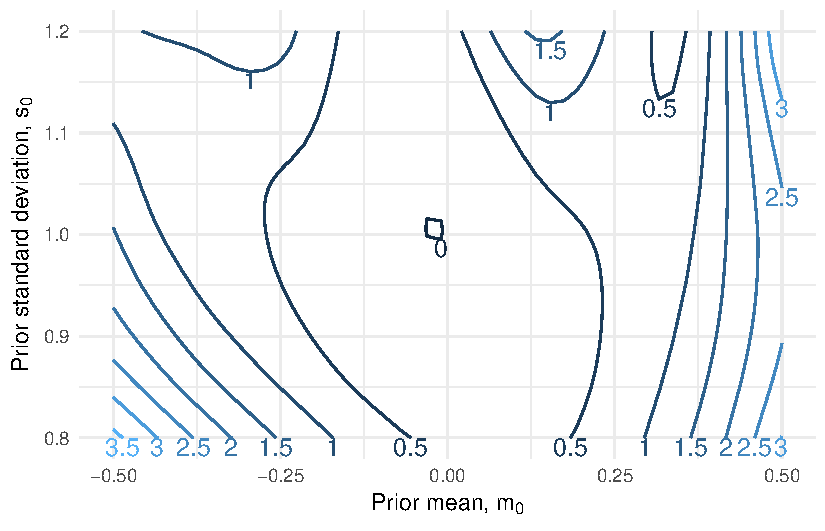
\includegraphics[scale=0.8]{./figures/sens_p.pdf}
\caption{Amount of regret when using the proposed OK-Diabetes programme design as the prior mean $m_0$ and prior standard deviation $s_0$ vary. }
\label{fig:sens_p}
\end{figure} 
%Contours are generated by fitting a generalised additive model with tensor product smooth term to a 500 point space-filling Sobol sequence experimental design.

Figure \ref{fig:sens_p} plots the regret over a range of prior means $m_0$ and prior standard deviations $s_0$. We varied the prior mean from -0.5 to 0.5, moving from extremely sceptical to enthusiastic beliefs. We find that over this range there is little to be gained from moving from the proposed design to the optimal design, providing the prior standard deviation is equal to or greater than the initial choice of $s_0 = 0.6$. As we decrease $s_0$ down to 0.48 the penalty of using the proposed design can increase, but the magnitude of these penalties depends on $m_0$. From these results we can conclude that the proposed design is quite robust to misspecification of the prior distribution, in the sense that if the choices of $m_0, s_0$ are not quite an accurate reflection of our prior beliefs, the design will still have an expected utility close to that of the true optimal design.

\begin{figure}
\centering
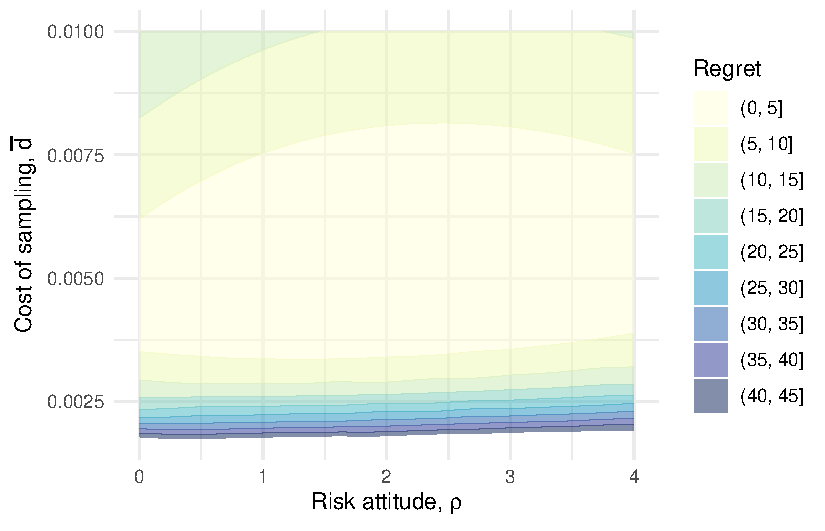
\includegraphics[scale=0.8]{./figures/sens_u.pdf}
\caption{Amount of regret when using the proposed OK-Diabetes programme design as the attitude to risk $\rho$ and cost of sampling $\bar{d}$ vary.}
\label{fig:sens_u}
\end{figure}
%Contours are generated by fitting a generalised additive model with tensor product smooth term to a 500 point space-filling Sobol sequence experimental design.

Corresponding results for varying utility parameters $\rho$ and $\bar{d}$ are given in Figure \ref{fig:sens_u}. We see that the proposed design is quite robust to misspecification of the attitude to risk, and to underestimation of the cost of sampling. However, if the cost of sampling is initially overestimated, the proposed design can become considerably sub-optimal. For example, maintaining $\rho = 2$ but halving the cost of sampling from 0.005 to $\bar{d} = 0.0025$ means the proposed design is worse than the true optimal design by an amount equivalent to 24 participants. This analysis suggests that the choice of $\bar{d}$, in particular, should be carefully examined to ensure it is a true reflection of the decision-maker's preferences.

\section{Evaluation}\label{sec:evaluation}

In the OK-Diabetes example we found that the standard policy of not testing for efficacy in an external pilot trial can be considerably sub-optimal. Here, we consider a range of different utility function parameter values and examine when, if at all, not testing in the pilot trial is optimal. Throughout, we maintain the same archetypal sceptical prior with $m_0 = 0$ and $s_0 = 0.6$. We considered the nine scenarios formed by setting the cost of sampling $\bar{d}$ to one of $\{0.0025, 0.005, 0.01\}$, and the treatment cost parameter $\hat{d} $ to one of $\{0.1, 0.2, 0.3\}$. For each of the nine scenarios we varied the attitude to risk, with $\rho \in [-5, 5]$, finding optimal programme designs over this range. We did this for two cases: firstly, assuming that a pilot sample size of $n_1 \geq 30$ is required in order to address feasibility questions; and secondly, removing this lower bound.

\subsection{The case $n_1 \geq 30$}

The results are given in Figure \ref{fig:eval}, which plots how the error rates of both the pilot ($i = 1$) and definitive ($i = 2$) trials vary with $\rho$, for each of the nine scenarios. In the scenarios considered, it is always optimal to test for effectiveness in the pilot trial, although the type I error rate used can be quite high. The largest we found was $\alpha_1 = 0.89$, when $\rho = -1.8, \bar{d} = 0.0025$ and $\hat{d} = 0.1$ (top left panel in Figure \ref{fig:eval}). The trends in Figure \ref{fig:eval} suggest that decreasing $\bar{d}$ and/or $\hat{d}$ could potentially lead to higher $\alpha_1$, but we failed to find any case where $\alpha_1 = 1$. Note that although $\alpha_1$ is found to be increasing as $\rho$ decreases in all scenarios (for sufficiently low $\rho$), and so we might expect there to be some negative $\rho$ such that $\alpha_1 = 1$, these scenarios also have $n_2 = 0$. That is, the pilot trial is the only trial being conducted.

\begin{figure}
\centering
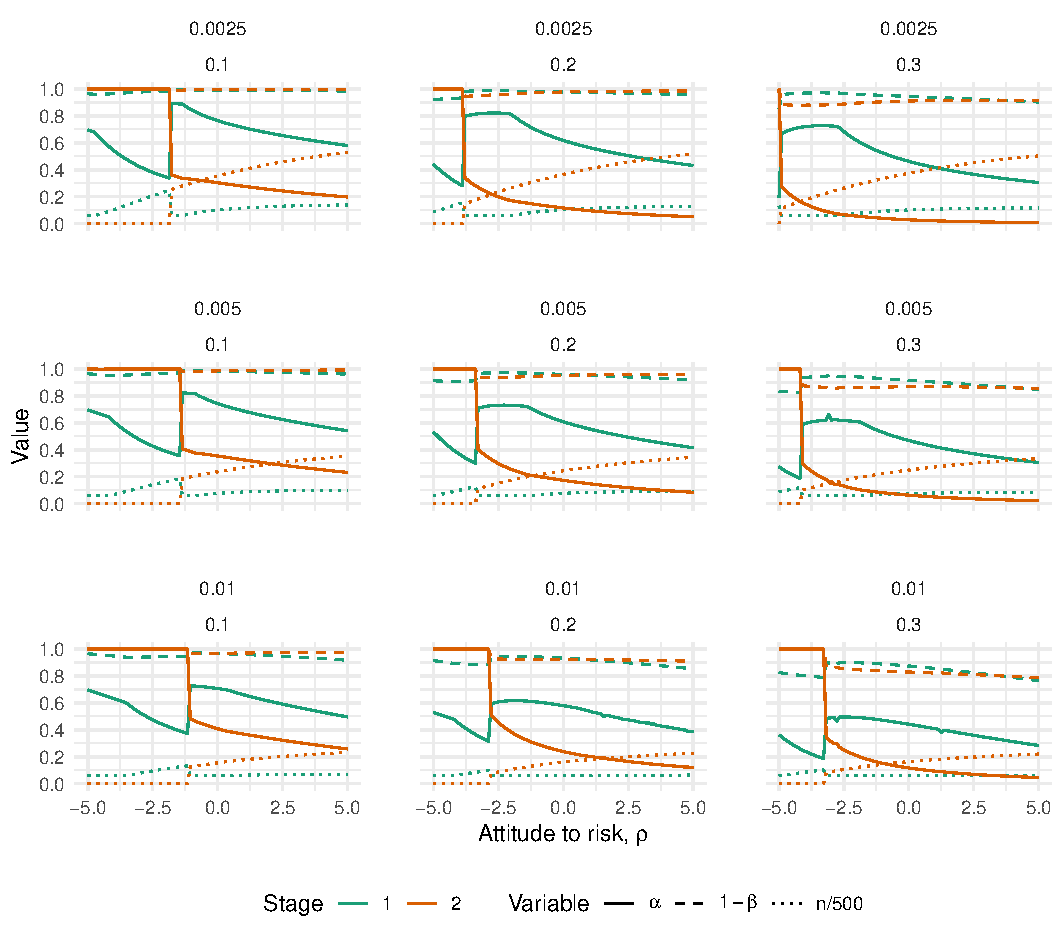
\includegraphics[scale=0.8]{./Figures/eval_np30.pdf}
\caption{Optimal type I error rates (solid lines), type II error rates (dashed lines) and scaled sample size (dotted lines) for varying values of $\rho$ (the attitude to risk, where higher means more risk-averse), when the pilot sample size is constrained to $n_1 \geq 30$.. Plots vary horizontally with treatment costs, $\hat{d} \in \{0.1, 0.2, 0.3\}$, and vertically with sampling costs, $\bar{d} \in \{0.0025, 0.005, 0.01\}$.}
\label{fig:eval}
\end{figure}

The broad trends which emerge from Figure \ref{fig:eval} are that optimal type I errors tend to decrease as we become more risk-averse, while optimal type II errors stay relatively stable. As the treatment costs increase (moving from left to right in Figure \ref{fig:eval}), both type I and II errors tend to decrease. And, as the cost of sampling increases (moving from top to bottom in Figure \ref{fig:eval}), both type I and II errors tend to decrease. In all nine scenarios we find there is a point where the definitive trial jumps to a design of $n_2 = 0, \alpha_2 = 1, 1-\beta_2 = 1$, meaning the pilot trial is the only trial which will be run. The point where this happens is always for a negative value of $\rho$. That is, there is a point where a sufficiently risk-seeking attitude will imply the optimal action is to run only one trial.

\subsection{The case $n_1 \geq 0$}

We now examine the characteristics of optimal programmes with no lower bound on the sample size at the pilot stage. This will be the case when the purpose of the pilot trial is only to assess effectiveness, as opposed to feasibility, and is similar to the problems considered in related work on optimal pilot design \cite{Stallard2012}. The results are given in Figure \ref{fig:eval2}, which plots how the error rates of both the pilot ($i = 1$) and definitive ($i = 2$) trials vary with $\rho$, for each of the nine scenarios.

\begin{figure}
\centering
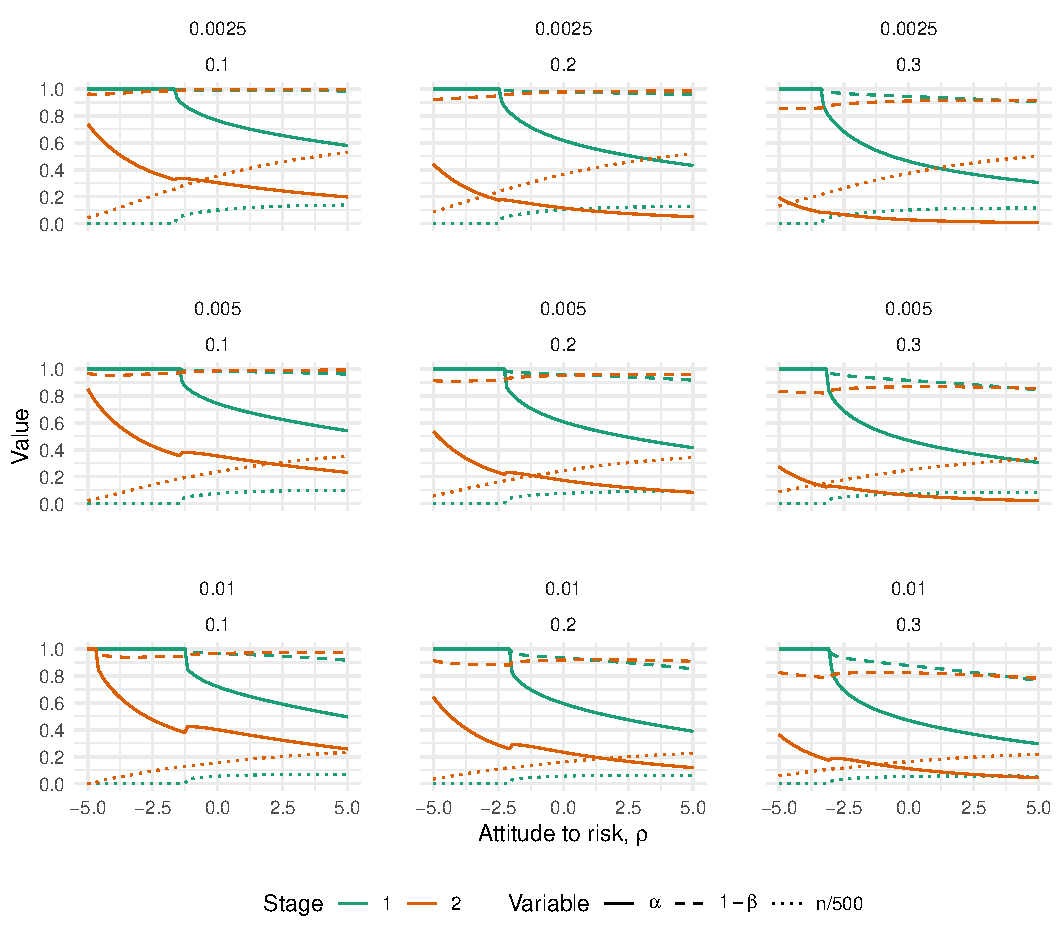
\includegraphics[scale=0.8]{./Figures/eval_unrest.pdf}
\caption{Optimal type I error rates (solid lines), type II error rates (dashed lines) and scaled sample size (dotted lines) for varying values of $\rho$ (the attitude to risk, where higher means more risk-averse), when the pilot sample size is unconstrained. Plots vary horizontally with treatment costs, $\hat{d} \in \{0.1, 0.2, 0.3\}$, and vertically with sampling costs, $\bar{d} \in \{0.0025, 0.005, 0.01\}$.}
\label{fig:eval2}
\end{figure}

The trends of how optimal error rates and sample sizes vary with the utility function parameters are broadly similar to those shown in Figure \ref{fig:eval}. We see similar inflection points, where now a sufficiently risk-seeking attitude will result in an optimal pilot trial sample size of $n_1 = 0$, leaving one one trial to be conducted. Optimal pilot trial type I error rates are only found to be $\alpha_1 = 1$ when $n_1 = 0$. In the scenarios considered here, we again fail to find a situation where it is optimal to run a pilot trial, but not test for effectiveness.

%Want to think about where it will fall down. Biggest concern would be the pilot introducing bias, probably positive, due to the idealised conditions. So, want to find optimal design when we have a bivariate normal prior on the treatment effect. Could have perfect correlation (i.e. known, fixed difference) which would give more of a sensitivity analysis; or could have a noisy relationship, which we would have to elicit. Computations are still OK - just integrating over a bivariate normal now, so can still use quadrature rules. Is there a connection here with surrogate endpoints? e.g. consider eliciting a treatment effect at 2 years, then working back to elicit the effect at two months (the pilot outcome). Need to elicit both the mean effect at each stage / outcome, but also the correlation. For correaltion, would need to ask questions like "if you found out the pilot true diff was X, what would you then think the main diff will be? Equiv to asking how much uncertainty will be left, gven estimated outcome diff. 

%Is this an evaluation of the robustness of the method, or an extension to allow fr a more general problem? More the former, but automatically provides everything we need for the latter. Put in illustration, as it's an example of how we would tackle a real problem. Define an example alternative prior and find the optimal design and compare. Want to understand how wrong using the original design would be - so measure utility diff and then translate into mu.

%In fact, this could be considered a special case of the more general issue of prior specification. So, after we get our design we might want to check if others would agree, and by how much; but crucially, we can let others use their own specific priors if we have some easy to use software.


\section{Extensions}\label{sec:extensions}

\subsection{Main trial}

In a sense a simplification, we should note that the method applies equally well to the case of a single confirmatory trial. We could place this in the context of other work talking about balancing error rates, e.g. \cite{Grieve2015, Walley2021} and references therein. The extension component comes from the closed form solution for expected utility (for the known variance case at least), which we can put in the appendix. Could apply to an example in the SM.

\subsection{Non-inferiority}

Although we have focussed on superiority trials, the decision-theoretic approach extends naturally to the non-inferiority setting. In a non-inferiority trial we are interested in testing whether or not the new intervention is not worse than the control by some pre-specified amount (the non-inferiority margin). The proposed method encompasses this setting by allowing for negative choices of the parameter $\hat{d}$, which denotes the amount of treatment difference we would consider equivalent to the costs of adopting the new treatment. In the non-inferiority setting the new treatment will be considered cheaper (in some sense, not necessarily monetary) than the control, leading to a negative $\hat{d}$.

As an example, we return to the OK-Diabetes trial of Section \ref{sec:illustration} but now consider tests of non-inferiority, where the non-inferiority margin is $\mu = -0.5$. Keeping all other parameters at their previous values but setting $\hat{d} = -0.3$, the optimal sample size at each stage is now $n_1 = 77, n_2 = 430$. The type I error rate is now defined as the probability of a positive test result conditional on the non-inferiority margin $\mu = -0.5$, while power is the probability of a positive test result conditional on no difference, $\mu = 0$. The optimal design then has error rates $\alpha_1 = 0.68, \beta_1 = 0.0057, \alpha_2 = 0.034, \beta_2 = 0.0011$.

\subsection{Internal pilots}

Internal pilot trials are distinguished from external pilots by their data being used at the final analysis, with a seamless gap between the pilot and definitive trial stages. Extending our problem to the internal pilot setting, we continue to conduct a first test based on the pilot sample mean difference $x_1$, but now follow this with a test of the overall sample mean difference $x_t$, where
$$
x_t = \frac{n_1 x_1}{n_1 + n_2} + \frac{n_2 x_2}{n_1 + n_2}.
$$
We can now apply equation \ref{eqn:joint_cond_util} in the internal pilot by defining $G_1 = x_1 > d_1$ and $G_2 = x_t > d_2$. The relevant probabilities can be calculated by noting that the pair $x_1, x_t$, conditional on $\mu$, follow a bivariate normal distribution. Specifically, the appendix will show that
$$
\begin{pmatrix}
x_1 \\
x_t
\end{pmatrix} \mid \mu
\sim BN\left( 
\begin{pmatrix}
\mu \\
\mu
\end{pmatrix},
\begin{pmatrix}
\frac{2\sigma^2}{n_1} & \frac{2\sigma^2}{n_1 + n_2} \\
\frac{2\sigma^2}{n_1 + n_2} & \frac{2\sigma^2}{n_1 + n_2}
\end{pmatrix} \right).
$$
The probabilities in equation \ref{eqn:joint_cond_util} are now with respect to this bivariate normal distribution, and can be calculated using (for example) the R package `mvtnorm' \cite{Genz2017}. Expected utility can then be calculated as before, integrating the conditional expected utility over the normal prior $p(\mu)$ using quadrature.

By way of illustration, we found the optimal internal pilot and definitive trial programme for the OK-Diabetes example. The details are provided in Table \ref{tab:ill_int}, where we also include the optimal programme for the external pilot case as found in Section \ref{sec:illustration}. Note that we summarise the programmes here in terms of the error rates of the pilot hypothesis test ($\alpha_1, \beta_1$) and the overall error rates of the programme ($\alpha_t, \beta_t$), as these are of more interest in the internal pilot setting. We find that the overall type I error rates are approximately equal for both the  external and internal pilot cases, and overall type II rates are very similar. The internal pilot programme has a slightly higher expected utility, which we might expect given the fact that all of the data is being utilised in the final analysis.

\begin{table}
\small\sf\centering
\caption{Optimal sample size and error rates for the OK-Diabetes pilot trial ($i = 1$) and subsequent definitive trial($i = 2$), when the pilot is external and internal.}
\input{./tables/ill_int.txt}
\label{tab:ill_int}
\end{table}



\subsection{Binary endpoint}

Suppose we have a binary primary endpoint, with probability of occurrence of $\tau_C$ in the control arm and $\tau_I$ in the intervention arm. We are interested in the absolute difference $\mu = \tau_C - \tau_I$, in the sense that this is what features in our utility. We use Beta priors to reflect our prior uncertainty, with $\tau_C \sim Beta(a_C, b_C)$ and $\tau_I \sim Beta(a_I, b_I)$.

We can extend our approach to this scenario by returning to equation \ref{eqn:joint_cond_util} and noting that, now conditioning on the pair of probabilities $(\tau_C, \tau_I)$, the probabilities of test success/failure at each stage can still be easily calculated. Now, rather than integrating the conditional expectation over a single normal prior density, we must integrate over the two independent beta distributions for $\tau_C$ and $\tau_I$. We can use general numerical integration methods such as the adaptive procedure implemented in the R package `cubature' \cite{Narasimhan2018} to estimate these integrals, although these will be slower than the Gauss-Hermite method used in the continuous case.

% This might be better in the discussion, where we can just note that the basic strategy can be easily applied to other models but that one of the difficulties will be in doing the integration. The other will be in specifying the utility, but we can't say much about that in general other than to use the same strategy of attributes - value - utility.

\subsection{Unknown variance}

When the variance of the primary outcome is unknown but still assumed to be common across arms, the tests at each stage of the design will compare $t$-statistics
$$
t_i = \frac{x_i}{\sqrt{2\hat{\sigma_i}^2 / n_i}}
$$
for stage $i = 1,2$, where $\hat{\sigma_i}^2$ are estimates of the variance at each stage. Conditional on $\mu, \sigma^2$, these $t$-statistics will follow non-central $t$-distributions with $2n_i - 2$ degrees of freedom and non-centrality parameter $\mu/\sqrt{2\sigma^2 / n_i}$. The probability of test success/failure at each stage in equation \ref{eqn:joint_cond_util} (now conditioning on $\mu$ and $\sigma^2$) can then be readily calculated. Given this conditional utility, we can proceed as before by numerically integrating over the prior distribution, now a joint prior $p(\mu, \sigma^2)$.

% We should implement this, even if only in the SM for a specific case, to make sure it is computationaly tractable. Should look at using nested quadrature over the gamma and normal dists. If this is fast and robust, it is worth saying so here.

%\subsection{Surrogate endpoints} We have assumed throughout that the endpoints at both stages are the same. Say we want to relax this, e.g. have the same continuous endpoint but measured earlier at the pilot stage. Closely related to the sensitivity analysis we do in the illustration, where we considered a positive bias in the pilot effect (but with the same endpoint at the same time). Key thing is that we need to elicit a bivariate distribution for the effect at both stages and the correlation between them. If we can do this, we can still use quadrature and everything will follow.

%\subsection{Two definitive trials} The FDA require as standard two statistically significant results from two different phase III trials for an intervention to be approved. If these are done simultaneously, assuming their optimal design is equal, can we modify our formulation? Same design parameters, same utility, but and additional set of trial realisation outcomes. Just need to change how we define stage 2 success $G_2$ - conditional on $\mu$, still easy to calculate (independent normals).

% Not considered for extensions here - multiple arms and multiple endpoints.

\section{Discussion}\label{sec:discussion}

% Summary and main implications
We have explored how Bayesian statistical decision theory can be used to define optimal type I and II error rates for trial programmes involving a pilot trial and a subsequent definitive trial. We have introduced a general utility function, outlining the associated assumptions, and demonstrated how its parameter values can be determined. When evaluating the conventional approach to pilot trial analysis, we found that a policy of not testing effectiveness was consistently sub-optimal. As a result, we recommend that pilot data can and should be used to conduct a preliminary test of effectiveness prior to the definitive trial, when the assumptions described in this paper hold. This would lead to a considerable improvement in the complex intervention evaluation pathway, as more ineffective interventions are identified at the pilot stage.

A key component of the decision-theoretic approach is the utility function. For simplicity, we did not include any set-up costs relating to the pilot or definitive trial. If these are thought to be important, expressing them in units of sample size would allow them to be included in the model easily. In terms of the resulting effect on optimal design characteristics, set-up costs would mean a design with either $n_1 = 0 $ or $n_2 = 0$ becoming more attractive. As such, we might expect to see such designs becoming optimal over a larger range of values for $\rho$ in Figures \ref{fig:eval} and \ref{fig:eval2}. We did not attempt to predict the number of patients who will be affected by the results of the definitive trial, or the manner in which they will adopt the intervention following a significant result. Were such a model to be included, the utilities of the people participating in the trial could be included and balanced against the utilities of those who stand to benefit from the trial results. Such considerations will be particularly important in small population contexts, such as with rare diseases, where the trial population can form a considerable fraction of the overall target population \cite{Pearce2018}. 

The exponential form of the utility function was based on an additive value function and an assumption of utility independence, in addition to an assumed mutual preferential independence between the three attributes. Although the appropriateness of these assumptions must be judged in light of the problem at hand, we note that an additive utility function is often assumed in related decision-theoretic work \cite{Gittins2000a, Willan2005, Kikuchi2009, Hee2012, Pearce2018} . As shown in equation \ref{eqn:expo_util}, an additive utility entails these assumptions while also assuming risk-neutrality on the part of the decision maker. It could be argued that the function $v_d(d)$ would actually take a non-linear form, with diminishing returns as $d$ increases. This will depend on the specific clinical context, but we note that in practice our assumption only requires linearity over the plausible region of $d$, as specified by the prior $p(\mu)$, which may be more reasonable. 

We have assumed throughout that the effect being measured is the same at both the pilot and definitive trial stages. One argument against assessing effectiveness in a pilot trial is that it may lead to a biased effect estimate \cite{Sim2019}. For example, it may be that the treatment providers involved at the pilot stage are likely to be more specialised, or more enthusiastic, than those who will be involved at the definitive stage. The methods proposed should, therefore, be used only when the pilot trial is an accurate reflection of the definitive trial. If it is thought that there will be some systematic difference, this could potentially be modelled in the Bayesian framework by introducing a bias parameter in the model and describing a prior distribution for it. In the extreme case where the amount of bias is completely unknown, the pilot data will be uninformative for the true treatment effect and testing at the pilot stage should be avoided.

%Operationally,  we are required to elicit the specific parameters describing the prior and utility from the decision maker. For the former, we can use methods based on summarising historical evidence (REF) or by eliciting expert opinions using, for example, the SHELF framework \cite{Dallow2018}. For the latter, we have described the types of questions which must be asked to determine values, and illustrated how a sensitivity analysis of these choices can be conducted.

% Extending to other scenarios

We have considered programmes where a hypothesis test is used in the primary analysis of the pilot and definitive trials. Further work could explore how a Bayesian analysis of pilot trial data could be used to update prior beliefs and use the revised knowledge to optimise the subsequent definitive trial. At the programme design stage, the pilot trial sample size could then be determined using value of information methods \cite{Willan2005}. A potential difficulty with such an approach is the computational aspect of such calculations, although techniques for enabling fast calculation of the expected value of sample information may be useful in this context \cite{Strong2015, Heath2019}. 

We have focussed on using pilot trials to test the efficacy of the intervention. Typically, pilot trials are used to estimate other parameters relating to the feasibility of the definitive trial, such as recruitment, follow-up and adherence rates \cite{Avery2017}. Learning about these parameters is clearly of value, and this value could be included in our utility formulation to be offset against the cost of sampling.

The optimisation problem \ref{eqn:opt} is not trivial, and we found some variability in performance of different optimisation algorithms. The suggested method was found to be robust, but it would be advisable to check for global convergence when applying to a given problem. This could be done by using other algorithms to check they agree or by using different starting points. Alternatively, several closely related problems could be solved and the resulting optimal programme characteristics plotted, much as we have done in the sensitivity analyses of Section \ref{sec:sensitivity}. We would expect to see smooth variation, with any erratic behaviour would suggest some convergence issues. Note this is exemplified in Figure \ref{fig:eval2}, where some small blips in the operating characteristic curves can be seen and would suggest a slight failure in convergence at these points.

%The utility function we have proposed has a simple form due to the various assumptions made regarding preferences within and between the three attributes of interest. As can be seen in Equations \ref{eqn:joint_cond_util} and \ref{eqn:exp_util}, the calculation and optimisation of expected utility would extend naturally to other utility functions (although note that the exact expected utility equation in the appendix would not). 

%Recall that we assumed identity value functions for the three attributes only to avoid cluttering the notation. We can simply replace the terms with the proper value functions and the general method will still hold. Thus, we can include situations where, for example, there is a concave value function on change in primary outcome (less benefit accruing as it increases). More generally, need to give people an idea of what they can change. So, can remove anything trivially. Can add deterministic attributes whose value depend only on the test results, e.g. set-up costs, trivially. Can't add attributes with uncertain parameters without a more thoughtful extension. Can generalise the utility we have by using non-identity value functions but keeping the additive form - so maintaining the same assumptions about preference independence etc. If we don't have preference independence we would need multi-linear or nonlinear value functions, wouldn't have the exponential utility result, and would need a much more involved elicitation process.

% The broader context
The motivation for our approach is the lack of guidance on how to balance the sample size and the type I and II error rates when testing in a pilot trial. The problem is by no means limited to the pilot trial setting, but for larger studies it tends to be `solved' by constraining type I and II error rates at default levels, typically $\alpha \leq 0.05$ (two-sided) and $\beta \leq 0.2$. Recently, much debate has focussed on if and how the default type I error rate should be changed \cite{Benjamin2017}, or abandoned altogether \cite{Amrhein2017, Lakens2018, Amrhein2019}; and similarly with the case of power thresholds \cite{Bacchetti2019}.



\begin{acks}
Acknowledgements.
\end{acks}

\begin{dci}
The Authors declare that there is no conflict of interest.
\end{dci}

\begin{funding}
This work was supported by the Medical Research Council [grant number MR/N015444/1].
\end{funding}

\bibliographystyle{SageV}
\bibliography{C:/Users/meddwilb/Documents/Literature/Databases/DTWrefs}

\section*{Appendix}

\subsection*{Expected utility for a single trial}

The utility function is $u(\mu, x)$, where $\mu$ is the true difference and $x$ is the sample mean difference. Note that
$$
x \mid \mu \sim N\left(\mu, \frac{2\sigma^2}{n} \right).
$$
Given a normal prior $\mu \sim N(\mu_0, \sigma_0^2)$, the posterior distribution of $\mu$ is also normal. Specifically
$$
\mu \mid x \sim N \left( \mu_1 = \sigma_1^2 \left( \frac{\mu_0}{\sigma_0^2} + \frac{xn}{2\sigma^2} \right), ~ \sigma_1^2 = 1/\left( \frac{1}{\sigma_0^2} + \frac{n}{2\sigma^2} \right) \right).
$$
The marginal distribution of the sample mean difference is
$$
x \sim N\left(\mu_0, \sigma_x^2 = \sigma_0^2 + \frac{2\sigma^2}{n} \right).
$$

For the case $\rho = 0$, the utility function is the value function. The expected utility is then
\begin{align*}
E[u(\mu, x)] =& E_x\left[ E_{\mu | x} [u(\mu, x)] \right] \\
=& E_x \left[ I\{x > d\} (k_d \mu_1 + k_n n) + I\{x \leq d\} (k_n n + k_c) \right] \\
=& k_n n + Pr(x > d) k_d E_{x | x > d} \left[ \mu_1 \right] + Pr(x \leq d)k_c,
\end{align*}
The two probabilities follow from the marginal distribution of the sample mean. For example,
$$
Pr[x > d] = 1- \Phi\left(\frac{d-\mu_0}{\sqrt{\sigma_0^2 + \frac{2\sigma^2}{n}}} \right)
$$
The expectation is of $\mu_1$, the mean of the posterior distribution on $\mu$ given $x$, with respect to the distribution of $x$ conditional on $x > d$. This is a truncated normal with mean
$$
E_{x | x > d} \left[ \mu_1 \right] = \mu_0 + \sigma_x \phi\left(\frac{d - \mu_0}{\sigma_x} \right)/\left(1 - \Phi\left(\frac{d - \mu_0}{\sigma_x}\right) \right).
$$

For the case $\rho > 0$, we again start with the law of total expectation giving $E[u(\mu, x)] = E_x\left[ E_{\mu | x} [u(\mu, x)] \right]$. Then,
\begin{align*}
E_{\mu | x} [u(\mu, x)] &= E_{\mu | x}[1 - e^{-\rho(k_d\mu + k_n n) I\{x > d\} -\rho(k_n n + k_c) I\{x < d\}}] \\
&= I\{x > d\} E_{\mu | x}[1 - e^{-\rho(k_d\mu + k_n n)}] + I\{x < d\}E_{\mu | x}[1 - e^{-\rho(k_n n + k_c)}]
\end{align*}
For the first term we have:
$$
E_{\mu | x}[1 - e^{-\rho(k_d\mu + k_n n)}] = 1 - e^{-\rho k_n n} E_{\mu | x}[e^{-\rho k_d \mu}]
$$
This takes the form as a moment generating function: for a normally distributed $Y \sim N(a, b^2)$,
$$
E[e^{tY}] = e^{ta + \frac{b^2 t^2}{2}}.
$$
This gives us
$$
E_{\mu | x}[1 - e^{-\rho(k_d\mu + k_n n)}] = 1 - e^{-\rho k_n n} \left(e^{t\mu_1 + \frac{\sigma_1^2 t^2}{2}} \right),
$$
where $t = \rho k_d$. This then all gives an expected utility conditional on $x$ of
$$
E_{\mu | x} [u(\mu, x)] = I\{x > d\} \left[1 - e^{-\rho k_n n} \left(e^{t\mu_1 + \frac{\sigma_1^2 t^2}{2}} \right) \right] + I\{x < d\}\left[1 - e^{-\rho(k_n n + k_c)}\right].
$$
We now need to take the expectation of this over the marginal distribution for $x$:
$$
\begin{aligned}
E[u(\mu, x)] &= E_x\left[ E_{\mu | x} [u(\mu, x)] \right] \\
 &= E_x\left[ I\{x > d\} \left(1 - e^{-\rho k_n n} e^{t\sigma_1^2(\frac{\mu_0}{\sigma_0^2} + \frac{xn}{2\sigma^2}) + \frac{\sigma_1^2 t^2}{2}} \right) \right] + 
 E_x\left[ I\{x < d\}\left(1 - e^{-\rho(k_n n + k_c)}\right) \right].
\end{aligned}
$$
The first term is equal to
$$
Pr[x > d] \left( 1 - e^{-\rho k_n n} e^{\frac{\sigma_1^2 t^2}{2}} e^{\frac{t\sigma_1^2 \mu_0}{\sigma_0^2}}   \right) E_x \left[ e^{\frac{t\sigma_1^2 x n}{2\sigma^2}} \right].
$$
For the expectation, we again use a moment generating function. Here, the sample difference $x$ is normally distributed $N(\mu_0, \sigma_x^2)$ but we have conditioned on $x > d$ and so have a truncated normal. The moment generating function for $Y \sim N(a,b^2), Y > d$ is
$$
E[e^{rY}] =  \left( e^{ar + \frac{b^2 r^2}{2} } \right) \left(\frac{1 - \Phi(\frac{d-a}{b} - br)}{1 - \Phi(\frac{d-a}{b} )} \right)
$$
So, for our case we have
$$
 E_x \left[ e^{\frac{t\sigma_1^2 x n}{2\sigma^2}} \right] = \left( e^{\mu_0 r + \frac{\sigma_x^2 r^2}{2} } \right) \left(\frac{1 - \Phi(\frac{d-\mu_0}{\sigma_x} - \sigma_x r)}{1 - \Phi(\frac{d-\mu_0}{\sigma_x})} \right),
$$
where $r = \frac{t \sigma_1^2 n}{2\sigma^2}$. Finally, putting everything together, we get
\begin{align*}
E[u(\mu, x)] =& E_x\left[ E_{\mu | x} [u(\mu, x)] \right] \\
 =& \left[ 1- \Phi\left(\frac{d-\mu_0}{\sqrt{\sigma_0^2 + \frac{2\sigma^2}{n}}} \right)  \right] \left[ 1 - e^{-\rho k_n n} e^{\frac{\sigma_1^2 t^2}{2}} e^{\frac{t\sigma_1^2 \mu_0}{\sigma_0^2}} \left( e^{\mu_0 r + \frac{\sigma_x^2 r^2}{2} } \right) \left(\frac{1 - \Phi(\frac{d-\mu_0}{\sigma_x} - \sigma_x r)}{1 - \Phi(\frac{d-\mu_0}{\sigma_x})} \right)  \right] + \\
 & \Phi\left(\frac{d-\mu_0}{\sqrt{\sigma_0^2 + \frac{2\sigma^2}{n}}} \right) \left[1 - e^{-\rho(k_n n + k_c)}\right].
\end{align*}
The case $\rho < 0$ follows.


\subsection*{Internal pilot sampling distribution}

Recall that we have sample means from both the first and second stage of an internal pilot design, $x_1, x_2$, with the combined sample mean $x_t = \frac{n_1 x_1}{n_1 + n_2} + \frac{n_2 x_2}{n_1 + n_2}$ being used at the final testing stage. The distribution of the combined mean, conditional on $\mu$ is $x_t \mid \mu \sim N\left( \mu, \frac{2\sigma^2}{n_1 + n_2} \right)$. To fully specify the joint distribution of $(x_1, x_t)$ we require the covariance:
$$
cov(x_1, x_t) = E[x_1 x_t] - E[x_1] E[x_t].
$$
By the law of total expectation,
\begin{align*}
E[x_1 x_t] &= E_{x_1} ( E_{x_1 x_t | x_1}[x_1 x_t] ) \\
&= E_{x_1} ( x_1 E_{x_t | x_1}[x_t] ) \\
&= E_{x_1} \left( x_1 E_{x_t | x_1}\left[\frac{n_1 x_1}{n_1 + n_2} + \frac{n_2 x_2}{n_1 + n_2}\right] \right) \\
&= E_{x_1} \left( \frac{n_1 x_1^2}{n_1 + n_2} + \frac{n_2 x_1 \mu}{n_1 + n_2} \right) \\
&= \frac{n_1}{n_1 + n_2} E[x_1^2] + \frac{n_2}{n_1 + n_2} E[x_1] \mu \\
&= \frac{n_1}{n_1 + n_2} (var(x_1) + E[x_1]^2) + \frac{n_2}{n_1 + n_2} \mu^2 \\
&= \frac{n_1}{n_1 + n_2} \left(\frac{2\sigma^2}{n_1} + \mu^2\right) + \frac{n_2}{n_1 + n_2} \mu^2.
\end{align*}
Then,
\begin{align*}
cov(x_1, x_t) &= \frac{n_1}{n_1 + n_2} \left(\frac{2\sigma^2}{n_1} + \mu^2\right) + \frac{n_2}{n_1 + n_2} \mu^2 - \mu^2 \\
&= \frac{2\sigma^2}{n_1 + n_2} + \frac{n_1 \mu^2}{n_1 + n_2} + \frac{n_2 \mu^2}{n_1 + n_2} - \mu^2 \\
&= \frac{2\sigma^2}{n_1 + n_2} .
\end{align*}




\subsection*{Partial derivatives of expected utility}

Denoting $Pr[G_i = 1 ~|~ \mu] = Pr[x_i > d_i 1 ~|~ \mu] = g(n_i, d_i)$ and $Pr[G_i = 0 ~|~ \mu] = Pr[x_i \leq d_i 1 ~|~ \mu] = \bar{g}(n_i, d_i)$ we can re-write the conditional expected utility of equation \ref{eqn:joint_cond_util} as
$$
\begin{aligned}
f(n_1,n_2,d_1,d_2) = &g(n_1,d_1)g(n_2,d_2) - g(n_1,d_1)g(n_2,d_2)\exp(-\rho(k_d\mu + k_n (n_1+n_2)) +\\
&g(n_1,d_1)\bar{g}(n_2,d_2) - g(n_1,d_1)\bar{g}(n_2,d_2)\exp(-\rho(k_n (n_1+n_2) + k_c)) + \\
&\bar{g}(n_1,d_1) - \bar{g}(n_1,d_1)\exp(-\rho(k_n n_1 + k_c)).
\end{aligned}
$$
Then, using the partial derivatives
$$
\frac{d}{dn_i} g(n_i,d_i) = \frac{d}{dn_i} \left[1 - \Phi \left(\frac{d_i-\mu}{\sqrt{2\sigma^2/n_i}} \right)\right] = -\phi\left(\frac{d_i-\mu}{\sqrt{2\sigma^2/n_i}} \right) \frac{d_i-\mu}{2\sqrt{2\sigma^2/n_i}}
$$
and
$$
\frac{d}{dd_i} g(n_i,d_i) = \frac{d}{dd_i} \left[1 - \Phi \left(\frac{d_i-\mu}{\sqrt{2\sigma^2/n_i}} \right)\right] = -\phi\left(\frac{d_i-\mu}{\sqrt{2\sigma^2/n_i}} \right) \frac{1}{\sqrt{2\sigma^2/n_i}},
$$
we can calculate the partial derivatives of the integrand in equation \ref{eqn:exp_util}. Given the quadrature approximation being used, the partial derivatives of the expected utility can then be calculated as the weighted sum of derivatives at the quadrature points. Full details can be found in the supplementary material.

\end{document}